\newpage
%%%%%%%%%%%%%%%%%%%%%%%%%%%%%%%%%%%%%%%%%%%%%%%%%%%%%%%%%%%%%%%%%%%%%%%%%%%%%%%
\section{Week 9?}
%%%%%%%%%%%%%%%%%%%%%%%%%%%%%%%%%%%%%%%%%%%%%%%%%%%%%%%%%%%%%%%%%%%%%%%%%%%%%%%
\subsection*{Monday, 07/17/2024}
\begin{itemize}
    \item man i can not count, but we are back. leptos rewrite going well,
        realized i need to use something like
        \texttt{\textcolor{blue}{\href{https://crates.io/crates/deadpool-diesel}{deadpool-diesel}}} since i
        already have some diesel endpoints i want to repurpose and apparently
        this deadpool crate integrates well with tokio (at least better than
        plain r2d2 from diesel)
    \item i will play around with this for article storage and more
    \item looks like deadpool is the move, will explore latest changes to crate
        and try to implement this over \texttt{r2d2}
    \item channels still sus as hell the way i use create_effect, but we will
        send it for now (i don't know how to use \texttt{loom} crate or similar yet to
        test async / concurrent stuff)
\end{itemize}

\subsection*{Tuesday, 07/18/2024}
\begin{itemize}
    \item i am getting skill issued when trying to convert to deadpool from
        vanilla postgres r2d2 setup haha. might just stick with what i had
        before and if the stream fails halfway by user refresh or anything else,
        that's just tough buddy\footnotemark
        \footnotetext{this will destroy me inside}
    \item wait, this \textit{is} possible with vanilla diesel, i was doing this 
        months ago since it was somehow easier than keeping track of each chunk 
        in a vector until the end haha
    \item ...
\end{itemize}

\subsection*{Wednesday, 07/19/2024}
\begin{itemize}
    \item finally got deadpool-diesel working and made a ding
        Figure~\ref{fig:fearless_concurrency}
        \begin{figure}[ht]
            \centering
            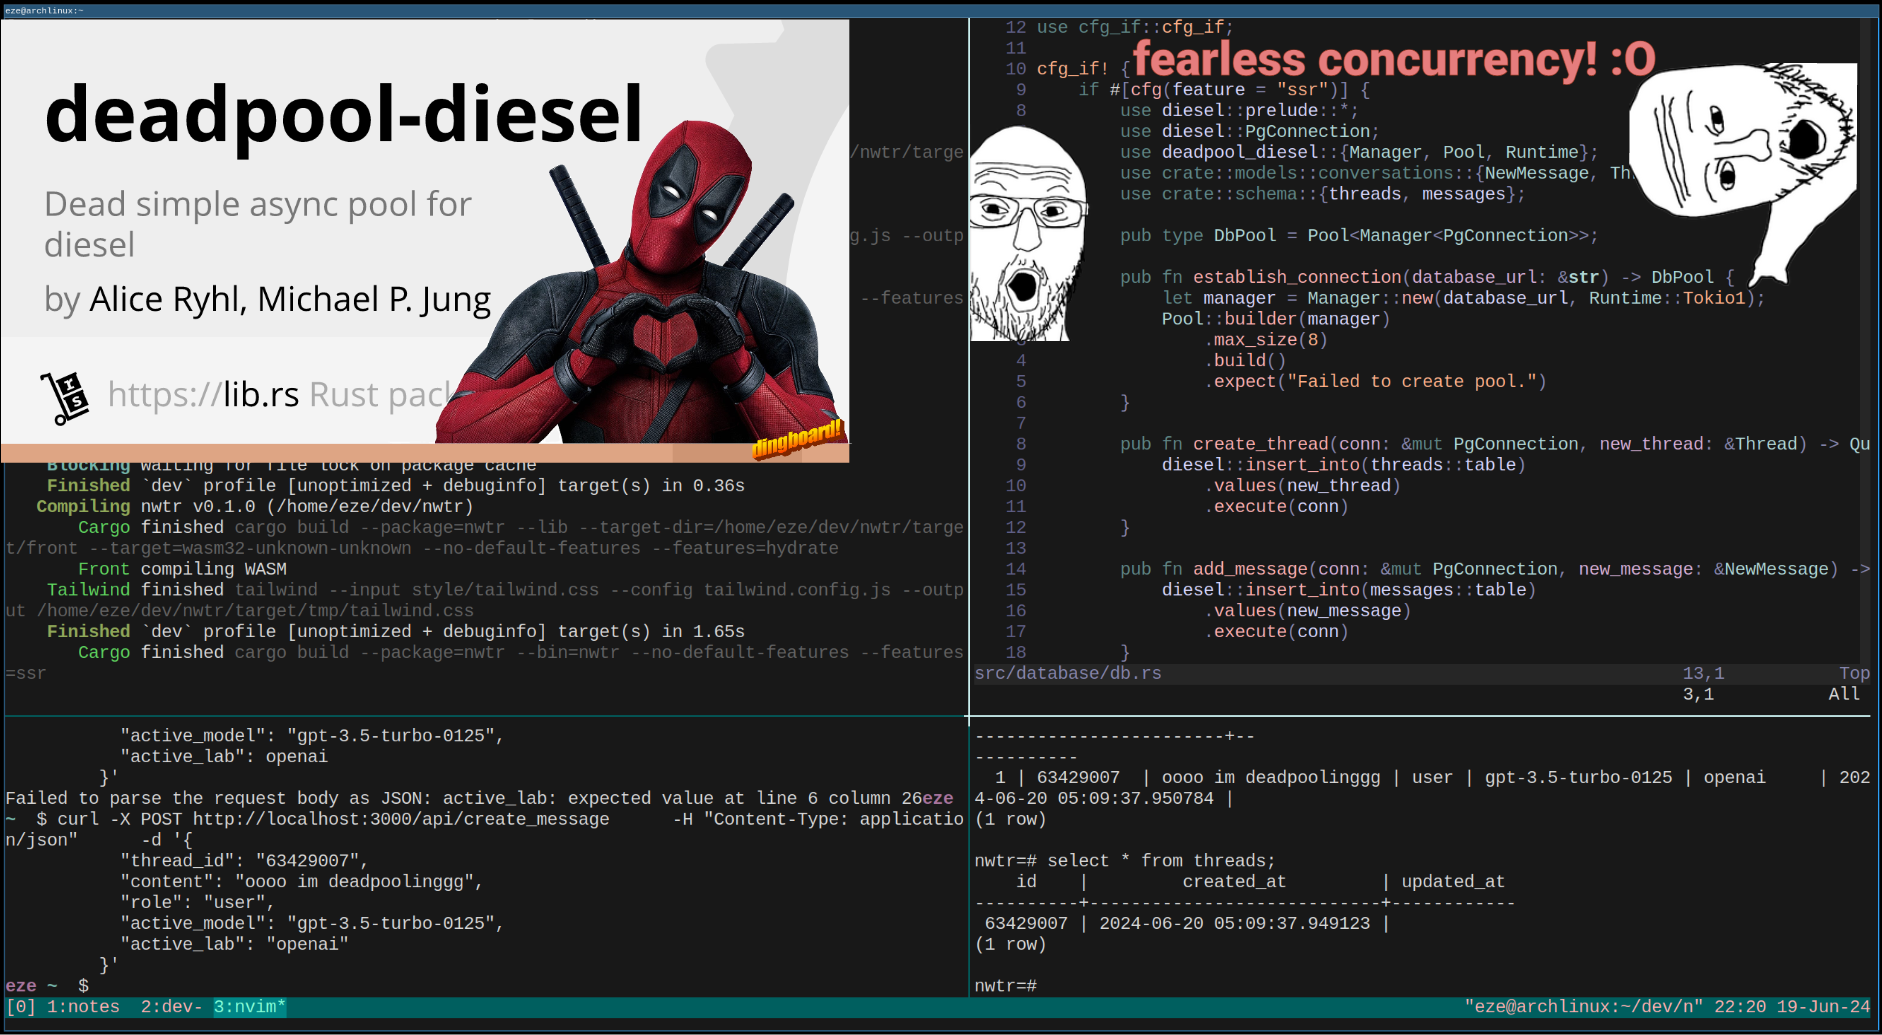
\includegraphics[width=15cm]{fearless_concurrency}
            \captionsetup{labelfont=bf, textfont=it}
            \caption{fearless concurrency !}
            \label{fig:fearless_concurrency}
        \end{figure}
\end{itemize}

\clearpage
\subsection*{Thursday, 07/20/2024}
\begin{itemize}
    \item added url encoding to allow user to upload code snippets or special
        characters basically. this should prevent bugs where a cast can have
        some strange character which breaks the request to create an article.
    \item we will see what the limits of what i can pass into the url for a get
        request can be. if this becomes an issue i can always change it up or
        even experiment with web sockets rather than sse if the complexity is
        not too crazy.
\end{itemize}
